This is a simple model that primarily serves as a way to verify the microscopic approach is working as expected by comparing with existing literature.
This approach can only model saturation concentrations, as the decay chain is not modeled.
It is called the 0D scaled model because it uses the scaled flux method, discussed in Section \ref{sec:bateman}.
The \gls{CFY} is used to calculate the equilibrium \gls{DNP} concentrations, with a scaling term based on the residence time of fuel salt in the core relative to the net residence time.
The \gls{CFY} gives the amount of each nuclide that is formed from both fission and decay.
An example solution with no reprocessing is shown in Equation \eqref{eq:cfy-conc} \cite{huynh2014calculation}:
\begin{equation}
    N_i = \frac{f_{in} CFY_i}{\lambda_i},
    \label{eq:cfy-conc}
\end{equation}
where
\begin{align}
    f_{in} &= \text{the fraction of time fuel-salt spends in the core [-]} \nonumber \\
    CFY_{i} &= \text{the cumulative fission yield of nuclide $i$ [-].} \nonumber
\end{align}
The derivation for this equation is given in Appendix \ref{sec:appendixB}.
It is important to note that the flux is scaled when calculating the fission rate as well, by the same $f_{in}$ term that scales the cumulative fission yield.
The $f_{in}$ term scaling the \gls{CFY} and fission rate cancels out when calculating the number of delayed neutrons per fission, which leads to no deviation in the results based on the residence time.

No cross-sections are included in this model, nor is time-dependent decay of nuclides into \glspl{DNP} included.
There is a possible approach to include the effects of \gls{DNP} absorption cross-sections in this model, but this approach is not used  \cite{shahbazi_steady-state_2022, benedictnuclear}.
The 0D flow model will account for absorption and transmutation cross-sections.

Figure \ref{fig:data-model} shows how the different data is loaded into \gls{MoSDeN}, including external data and user defined input data.
The green circles represent input data required for generating the \gls{DNP} group parameters.
The red diamond represents \gls{MoSDeN}.
\gls{MoSDeN} takes in the data to simulate irradiation of the target fissile sample to generate the irradiated concentrations, the delayed neutron count rate, and finally the \gls{DNP} group parameters that fit that count rate.
The blue squares represent the outputs, in this case the \gls{DNP} group parameters: the \gls{DNP} group yields and the \gls{DNP} group half-lives.

\begin{figure}[H]
    \centering
    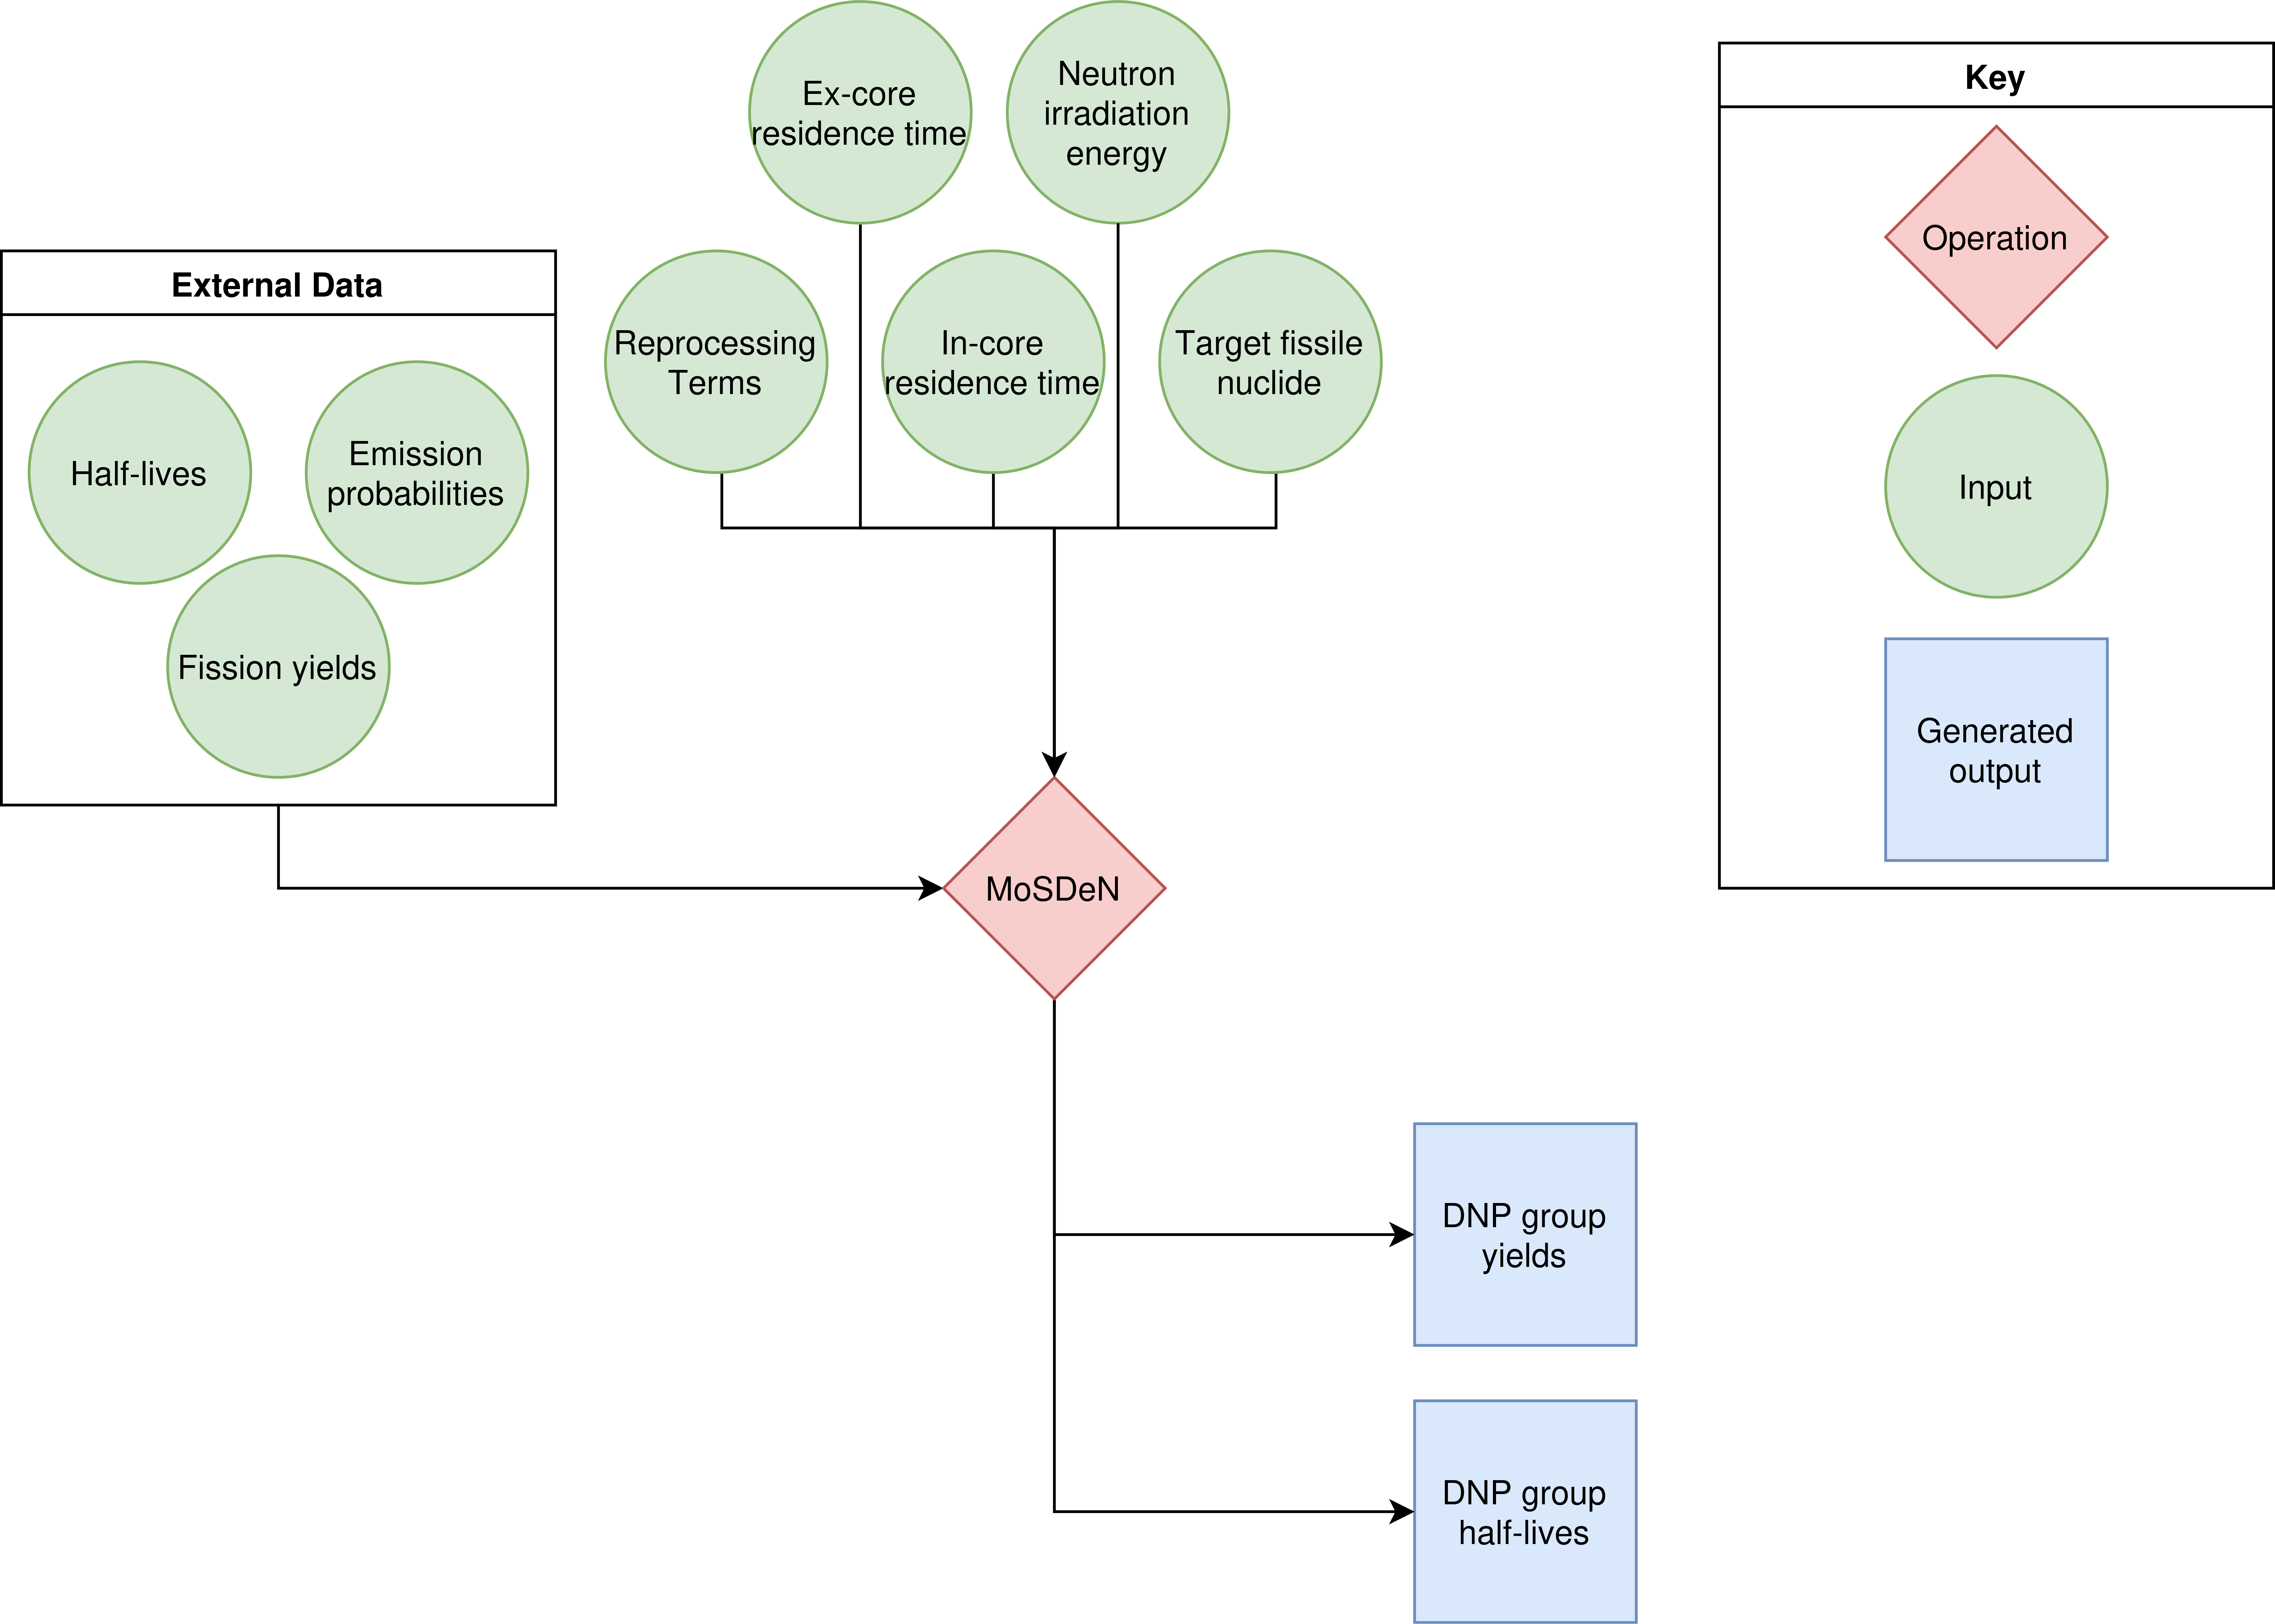
\includegraphics[width=0.9\linewidth]{images/data-driven.png}
    \caption{Flow diagram of 0D scaled model used to generate improved \gls{DNP} group parameters.}
    \label{fig:data-model}
\end{figure}

After all this data is loaded into \gls{MoSDeN}, it generates the concentration of each \gls{DNP}.
This concentration is then combined with emission probabilities and decay constants to form a delayed neutron count rate.
A non-linear least squares solve then fits the improved \gls{DNP} group parameters to the delayed neutron count rate, generating the group yields and half-lives, given as blue squares in Figure \ref{fig:data-model}.

This model is only valid for saturation irradiation simulations, as the concentration calculated in Equation \eqref{eq:cfy-conc} is the equilibrium concentration.
For a pulse irradiation, this approach is not valid.
This prevents the 0D scaled model from simulating pulse irradiations.
The proposed 0D flow model can simulate pulse irradiations, and it will be used to evaluate whether pulse irradiations provide more accurate yields and half-lives for the shorter-lived \glspl{DNP}.